% !TeX program = xelatex
\ifdefined\BookMaster\else
\documentclass[11pt,oneside]{article}
% !TeX program = xelatex
\usepackage[b5paper,left=22mm,right=22mm,top=20mm,bottom=22mm,footskip=11mm]{geometry}
\usepackage{fontspec}
\setmainfont{TeX Gyre Termes}
\setsansfont{TeX Gyre Heros}
\usepackage{amsmath,amssymb,mathtools,amsthm}
\renewcommand{\cdots}{\mathinner{\cdotp\cdotp\cdotp}}
\usepackage{graphicx,adjustbox,array,booktabs,longtable,multirow,enumitem,changepage,needspace}
\usepackage[table]{xcolor}
\usepackage{fancyhdr}
\raggedbottom
\interfootnotelinepenalty=10000
\newcommand{\BookFootnote}[2]{\begingroup\renewcommand{\thefootnote}{\fnsymbol{footnote}}\footnote[#1]{#2}\endgroup}
\newcommand{\BookFootnoteMark}[1]{\begingroup\renewcommand{\thefootnote}{\fnsymbol{footnote}}\footnotemark[#1]\endgroup}
\newcommand{\BookFootnoteText}[2]{\begingroup\renewcommand{\thefootnote}{\fnsymbol{footnote}}\footnotetext[#1]{#2}\endgroup}
\newenvironment{BookFloat}[1]{\par\addvspace{.6\baselineskip}\noindent\def\BookFloatID{#1}\begin{minipage}{\linewidth}\phantomsection\label{bookfloat:#1:start}}{\phantomsection\label{bookfloat:\BookFloatID:end}\end{minipage}\par\addvspace{.6\baselineskip}}

\usepackage[unicode,hidelinks]{hyperref}
\pagestyle{fancy}
\fancyhf{}
\newcommand{\BookFooter}{}
\fancyfoot[L]{\parbox[b]{\dimexpr\textwidth-15mm}{\footnotesize\BookFooter}}
\fancyfoot[R]{\footnotesize\thepage}
\renewcommand{\headrulewidth}{0pt}
\renewcommand{\footrulewidth}{0pt}
\setlength{\parindent}{0pt}
\setlength{\parskip}{0.2em}
\setlength{\emergencystretch}{3em}
\setlist{nosep,leftmargin=1.7em,labelsep=.65em}
\newif\ifBookNarrative
\BookNarrativetrue
\newenvironment{BookBody}{\setlength{\parindent}{0pt}}{}
\newcommand{\BookStatement}[1]{\par\addvspace{.6\baselineskip}\noindent #1\enspace\ignorespaces}
\newcommand{\BookLabel}[1]{\par\addvspace{.6\baselineskip}\needspace{3\baselineskip}\noindent\textbf{#1}\quad\ignorespaces}
\newcommand{\BookHeading}[1]{\par\addvspace{\baselineskip}\needspace{4\baselineskip}\noindent{\large\bfseries #1}\par\medskip}
\newcommand{\BookSubheading}[1]{\par\addvspace{.7\baselineskip}\needspace{3\baselineskip}\noindent{\bfseries #1}\par\smallskip}
\newcommand{\BookTextHeading}[1]{\par\addvspace{.7\baselineskip}\needspace{3\baselineskip}\noindent #1\par\smallskip}
\newcommand{\BookSectionTitle}[2]{\par\addvspace{1.2\baselineskip}\needspace{5\baselineskip}\noindent\colorbox{gray!25}{\sffamily\bfseries\small SECTION #1}\quad{\large\bfseries #2}\par\medskip}
\newcommand{\BookExerciseTitle}[1]{\par\addvspace{\baselineskip}\needspace{4\baselineskip}\noindent{\color{gray}\rule{1.5mm}{1.5mm}}\enspace{\large\bfseries Exercises #1}\par\medskip}
\newcommand{\BookBullet}[1]{\begin{list}{\textbullet}{\setlength{\leftmargin}{1.7em}\setlength{\labelwidth}{1em}\setlength{\labelsep}{.7em}\setlength{\topsep}{0pt}\setlength{\parsep}{0pt}\setlength{\itemsep}{0pt}}\item #1\end{list}}
\newcommand{\BookExercise}[2]{\begin{list}{\textbf{#1}}{\setlength{\leftmargin}{2.2em}\setlength{\labelwidth}{1.5em}\setlength{\labelsep}{.7em}\setlength{\topsep}{.15em}\setlength{\parsep}{0pt}\setlength{\itemsep}{0pt}}\item #2\end{list}}
\newcommand{\BookEnd}[1]{\unskip\nobreak\hfill\ensuremath{#1}}
\newcommand{\BookSource}[2]{\phantomsection\label{sourcepage:#1}} % Source-page anchors, retained through reflow.
\usepackage{multicol}
\usepackage{tikz}
\newcommand{\BookPartEntry}[2]{\par\noindent\makebox[17mm][l]{\bfseries Section #1}#2\par}
\newcommand{\BookPartTitle}[3]{\par\bigskip\noindent\begin{tikzpicture}\node[anchor=north west,inner sep=0pt,outer sep=0pt] (bookpart) at (0,0) {\begin{minipage}{\dimexpr\linewidth-.5pt}\hspace*{26mm}\begin{minipage}[t]{\dimexpr\linewidth-26mm}\begin{adjustbox}{max width=\linewidth}{\fontsize{20}{24}\selectfont\bfseries #2}\end{adjustbox}\par\vspace{6mm}\hrule\vspace{6mm}{\sffamily\footnotesize\setlength{\parskip}{.3em}#3}\vspace{3mm}\end{minipage}\end{minipage}};\path[shade,top color=gray!60,bottom color=white] (0,0) rectangle ([xshift=24mm]bookpart.south west);\node[anchor=north,font=\sffamily\bfseries\small] at (12mm,-2mm) {PART};\node[anchor=north,font=\sffamily\bfseries\Huge] at (12mm,-7mm) {#1};\end{tikzpicture}\par\bigskip}
\newsavebox{\BookMathBox}
\makeatletter
\newcommand{\BookInline}[1]{\leavevmode\hskip0pt\relax\begingroup\in@{\begin}{#1}\ifin@\sbox{\BookMathBox}{\(#1\)}\ifdim\wd\BookMathBox>\dimexpr\linewidth-1em\relax\resizebox{\dimexpr\linewidth-1em\relax}{!}{\usebox{\BookMathBox}}\else\(#1\)\fi\else\in@{\left}{#1}\ifin@\sbox{\BookMathBox}{\(#1\)}\ifdim\wd\BookMathBox>\dimexpr\linewidth-1em\relax\resizebox{\dimexpr\linewidth-1em\relax}{!}{\usebox{\BookMathBox}}\else\(#1\)\fi\else\(#1\)\fi\fi\endgroup\hskip0pt\relax}
\makeatother
\DeclareMathOperator{\Aut}{Aut}
\DeclareMathOperator{\End}{End}
\DeclareMathOperator{\Hom}{Hom}
\DeclareMathOperator{\GF}{GF}
\DeclareMathOperator{\irr}{irr}
\DeclareMathOperator{\lt}{lt}
\DeclareMathOperator{\lp}{lp}
\providecommand{\textcircled}[1]{\textnormal{(#1)}}

\begin{document}
\fi
\renewcommand{\BookFooter}{Front Matter}
\pdfbookmark[0]{Front Matter}{front_matter}
\ifdefined\BookMaster\else\pagenumbering{roman}\fi
% Source PDF page 1; original printed page 
\BookSource{1}{}
\begin{center}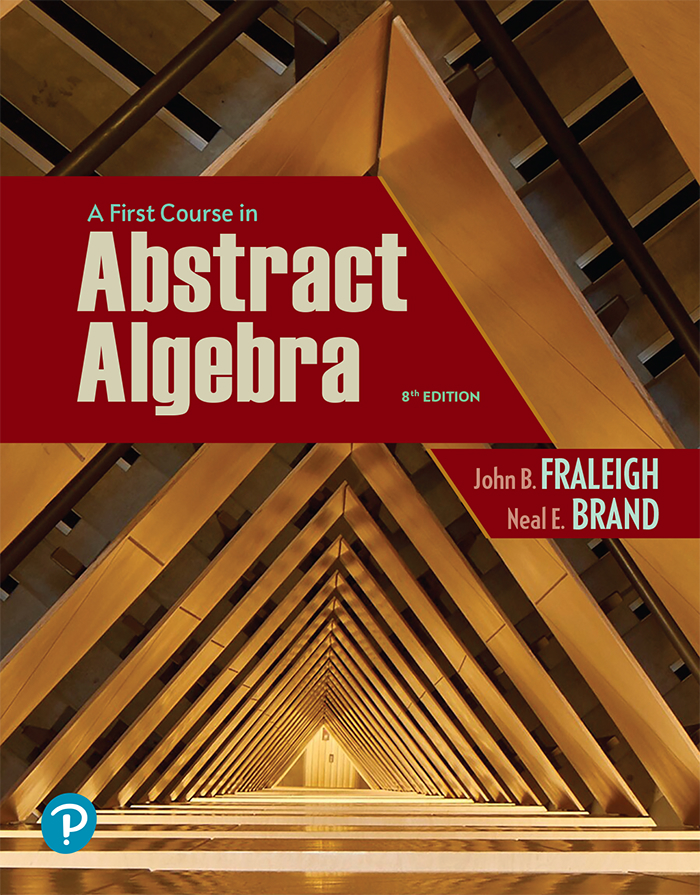
\includegraphics[width=0.960\linewidth,height=.8\textheight,keepaspectratio]{assets/front_001.pdf}\end{center}

% Source PDF page 2; original printed page 
\BookSource{2}{}
\begin{center}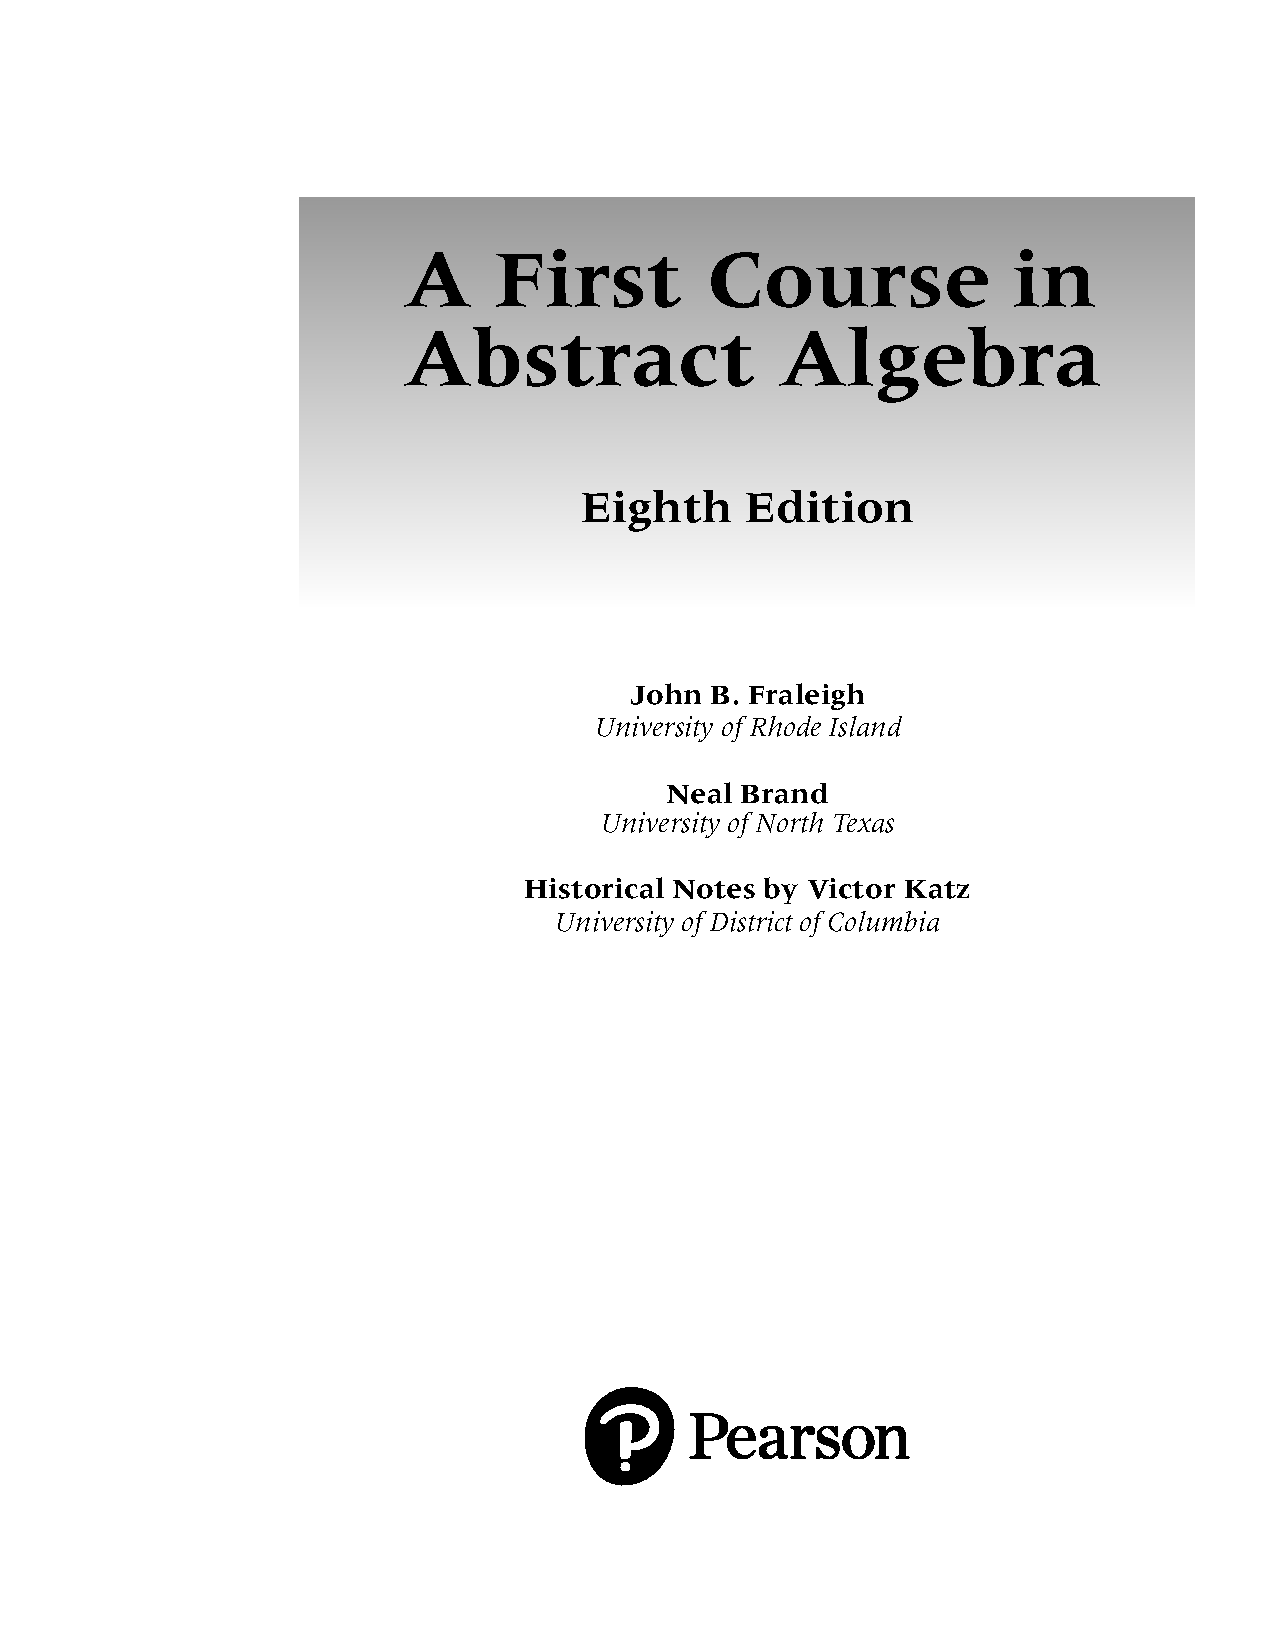
\includegraphics[width=1.000\linewidth,height=.8\textheight,keepaspectratio]{assets/front_002.pdf}\end{center}

% Source PDF page 3; original printed page 
\BookSource{3}{}
\BookNarrativefalse

\begin{BookBody}

\footnotesize

\noindent Copyright \BookInline{\text{\copyright} }c 2021, 2003, 1994 by Pearson Education, Inc. or its affiliates, 221 River Street, Hoboken, NJ 07030. All Rights Reserved. Manufactured in the United States of America. This publication is protected by copyright, and permission should be obtained from the publisher prior to any prohibited reproduction, storage in a retrieval system, or transmission in any form or by any means, electronic, mechanical, photocopying, recording, or otherwise. For information regarding permissions, request forms, and the appropriate contacts within the Pearson Education Global Rights and Permissions department, please visit \url{www.pearsoned.com/permissions/.}

\noindent Acknowledgments of third-party content appear on the appropriate page within the text.

\noindent Cover image credit: Edmund Sumner/AGE Fotostock

\noindent PEARSON, ALWAYS LEARNING, and MYLAB are exclusive trademarks owned by Pearson Education, Inc. or its affiliates in the U.S. and/or other countries.

\noindent Unless otherwise indicated herein, any third-party trademarks, logos, or icons that may appear in this work are the property of their respective owners, and any references to third-party trademarks, logos, icons, or other trade dress are for demonstrative or descriptive purposes only. Such references are not intended to imply any sponsorship, endorsement, authorization, or promotion of Pearson’s products by the owners of such marks, or any relationship between the owner and Pearson Education, Inc., or its affiliates, authors, licensees, or distributors.

\BookTextHeading{\textbf{Library of Congress Cataloging-in-Publication Data}  }

\noindent Names: Fraleigh, John B., author\BookInline{.|} Katz, Victor J., writer of added commentary.

\noindent Title: A first course in abstract algebra / John B. Fraleigh; historical notes by Victor Katz.

\noindent Description: Eighth edition\BookInline{.|[}Hoboken, New Jersey]: Pearson\BookInline{,\allowbreak [2021]|}

\noindent Series: World student series \BookInline{|} Includes bibliographical references and index.

\noindent Identifiers: LCCN \BookInline{2019038536|} ISBN 9780135758168 (paperback\BookInline{)\; |} ISBN 9780321390363 (ebook)

\noindent Subjects: LCSH: Algebra, Abstract.

\noindent Classification: LCC QA162.F\BookInline{72020|} DDC 512/.02–dc23

\noindent LC record available at \url{https://lccn.loc.gov/2019038536}

\noindent ScoutAutomatedPrintCode

Rental ISBN-10: 0-13-673162-7 ISBN-13: 978-0-13-673162-7

Loose Leaf Version

ISBN-10:

0-13-575816-5

ISBN-13: 978-0-13-575816-8

\end{BookBody}

% Source PDF page 4; original printed page 
\BookSource{4}{}
\BookHeading{Contents}
\begin{longtable}{@{}p{.83\linewidth}r@{}}
Instructor’s Preface & vii\\
Dependence Chart & xii\\
Student’s Preface & xv\\
0 Sets and Relations & 1\\
\textbf{I Groups and Subgroups} & 11\\
\hspace*{1em}1 Binary Operations & 11\\
\hspace*{1em}2 Groups & 19\\
\hspace*{1em}3 Abelian Examples & 32\\
\hspace*{1em}4 Nonabelian Examples & 39\\
\hspace*{1em}5 Subgroups & 52\\
\hspace*{1em}6 Cyclic Groups & 61\\
\hspace*{1em}7 Generating Sets and Cayley Digraphs & 70\\
\textbf{II Structure of Groups} & 77\\
\hspace*{1em}8 Groups of Permutations & 77\\
\hspace*{1em}9 Finitely Generated Abelian Groups & 88\\
\hspace*{1em}10 Cosets and the Theorem of Lagrange & 97\\
\hspace*{1em}\textsuperscript{\BookInline{\dagger}}\,11 Plane Isometries & 105\\
\textbf{III Homomorphisms and Factor Groups} & 113\\
\hspace*{1em}12 Factor Groups & 113\\
\hspace*{1em}13 Factor-Group Computations and Simple Groups & 121\\
\hspace*{1em}\textsuperscript{\BookInline{\ddagger}}\,14 Group Action on a Set & 132\\
\hspace*{1em}\textsuperscript{\BookInline{\dagger}}\,15 Applications of G-Sets to Counting & 140\\
\textbf{IV Advanced Group Theory} & 145\\
\hspace*{1em}16 Isomorphism Theorems & 145\\
\hspace*{1em}17 Sylow Theorems & 149\\
\hspace*{1em}18 Series of Groups & 157\\
\hspace*{1em}19 Free Abelian Groups & 166\\
\hspace*{1em}20 Free Groups & 172\\
\hspace*{1em}21 Group Presentations & 177\\
\textbf{V Rings and Fields} & 185\\
\hspace*{1em}22 Rings and Fields & 185\\
\hspace*{1em}23 Integral Domains & 194\\
\hspace*{1em}24 Fermat’s and Euler’s Theorems & 200\\
\hspace*{1em}25 Encryption & 205\\
\textbf{VI Constructing Rings and Fields} & 211\\
\hspace*{1em}26 the Field of Quotients of an Integral Domain & 211\\
\hspace*{1em}27 Rings of Polynomials & 218\\
\hspace*{1em}28 Factorization of Polynomials over a Field & 228\\
\hspace*{1em}\textsuperscript{\BookInline{\dagger}}\,29 Algebraic Coding Theory & 237\\
\hspace*{1em}30 Homomorphisms and Factor Rings & 243\\
\hspace*{1em}31 Prime and Maximal Ideals & 250\\
\hspace*{1em}\textsuperscript{\BookInline{\dagger}}\,32 Noncommutative Examples & 258\\
\textbf{VII Commutative Algebra} & 267\\
\hspace*{1em}33 Vector Spaces & 267\\
\hspace*{1em}34 Unique Factorization Domains & 275\\
\hspace*{1em}35 Euclidean Domains & 286\\
\hspace*{1em}36 Number Theory & 292\\
\hspace*{1em}\textsuperscript{\BookInline{\dagger}}\,37 Algebraic Geometry & 297\\
\hspace*{1em}\textsuperscript{\BookInline{\dagger}}\,38 Gröbner Bases for Ideals & 303\\
\textbf{VIII Extension Fields} & 311\\
\hspace*{1em}39 Introduction to Extension Fields & 311\\
\hspace*{1em}40 Algebraic Extensions & 319\\
\hspace*{1em}\textsuperscript{\BookInline{\dagger}}\,41 Geometric Constructions & 328\\
\hspace*{1em}42 Finite Fields & 335\\
\textbf{IX Galois Theory} & 341\\
\hspace*{1em}43 Introduction to Galois Theory & 341\\
\hspace*{1em}44 Splitting Fields & 349\\
\hspace*{1em}45 Separable Extensions & 357\\
\hspace*{1em}46 Galois Theory & 364\\
\hspace*{1em}47 Illustrations of Galois Theory & 372\\
\hspace*{1em}48 Cyclotomic Extensions & 378\\
\hspace*{1em}49 Insolvability of the Quintic & 384\\
Appendix: Matrix Algebra & 391\\
Bibliography & 395\\
Notations & 397\\
Answers to Odd-numbered Exercises Not Asking for Definitions or Proofs & 401\\
Index & 419\\
\end{longtable}
{\footnotesize\noindent \BookInline{\dagger} Not required for the remainder of the text.\par\noindent \BookInline{\ddagger} This section is a prerequisite for Sections 17 and 36 only.\par}

% Source PDF page 5; original printed page iv
\BookSource{5}{iv}


% Source PDF page 6; original printed page v
\BookSource{6}{v}


% Source PDF page 8; original printed page 
\BookSource{8}{}
\BookNarrativetrue

\begin{BookBody}

\BookTextHeading{\textbf{Instructor’s Preface}  }

\noindent This is an introduction to abstract algebra. It is anticipated that the students have studied calculus and probably linear algebra. However, these are primarily\textit{ mathematical ma}\textit{turity} prerequisites; subject matter from calculus and linear algebra appears mostly in illustrative examples and exercises.

As in previous editions of the text, our aim remains to teach students as much about groups, rings, and fields as we can in a first course. For many students, abstract algebra is their first extended exposure to an axiomatic treatment of mathematics. Recognizing this, we have included extensive explanations concerning what we are trying to accomplish, how we are trying to do it, and why we choose these methods. Mastery of this text constitutes a firm foundation for more specialized work in algebra and also provides valuable experience for any further axiomatic study of mathematics.

\BookTextHeading{\textbf{New to This Edition}  }

\noindent [Editor’s Note: You may have noticed something new on the cover of the book. Another author! I am thrilled that Neal Brand agreed to update this classic text. He has done so carefully and thoughtfully, staying true to the spirit in which it was written. Neal’s years of experience teaching the course with this text at the University of North Texas have helped him produce a meaningful and worthwhile update to John Fraleigh’s work.]

\BookTextHeading{\textit{\textbf{Updates for the eText}}  }

\noindent A focus of this revision was transforming it from a primarily print-based learning tool to a digital learning tool. The eText is therefore filled with content and tools that will help bring the content of the course to life for students in new ways and help you improve instruction. Specifically,

\BookBullet{\textbf{Mini lectures.} These brief author-created videos for each section of the text give an overview to the section but not every example or proof. Some sections will have two videos. I have used these videos effectively with my students, who were assigned to watch them ahead of the lecture on that topic. Students came to class with a basic overview of the topic of the day, which had the effect of reducing lecture time and increasing the class time used for discussion and student 
% Source PDF page 9; original printed page viii
\BookSource{9}{viii}
presentations. Students reported that the videos were helpful in giving an overview of the topics and a better understanding of the concepts and proofs. Students were also encouraged to view the videos after the topic was covered in class to reinforce what they learned. Many students also used the videos to review topics while preparing for exams. Although I have not attempted to flip the classroom, my intention was to provide sufficient resources in the eText to make it feasible without requiring other resources.}

\end{BookBody}

\BookNarrativetrue

\begin{BookBody}

\BookBullet{\textbf{Key idea quizzes.} A database of definitions and named theorems will allow students to quiz themselves on these key ideas. The database can be used in the way that flash cards were traditionally used.}

\BookBullet{\textbf{Self-assessments.} Occasional questions interspersed in the narrative allow students to check their understanding of new ideas.}

\BookBullet{\textbf{Interactive figures and utilities.} I have added a number of opportunities for students to interact with content in a dynamic manner in order to build or enhance understanding. Interactive figures allow students to explore concepts geometrically or computationally in ways that are not possible without technology.}

\BookBullet{\textbf{Notes, Labels, and Highlights.} Notes allow instructors to add their personal teaching style to important topics, call out need-to-know information, or clarify difficult concepts. Students can make their eText their own by creating highlights with meaningful labels and notes, helping them focus on what they need to study. The customizable Notebook allows students to filter, arrange, and group their notes in a way that makes sense to them.}

\BookBullet{\textbf{Dashboard.} Instructors can create reading assignments and see the time spent in the eText so that they can plan more effective instruction.}

\BookBullet{\textbf{Portability.} Portable access lets students read their eText whenever they have a moment in their day, on Android and iOS mobile phones and tablets. Even without an Internet connection, offline reading ensures students never miss a chance to learn.}

\BookBullet{\textbf{Ease-of-Use.} Straightforward setup makes it easy for instructors to get their class up and reading quickly on the first day of class. In addition, Learning Management System (LMS) integration provides institutions, instructors, and students with single sign-on access to the eText via many popular LMSs.}

\BookTextHeading{\textit{\textbf{Exercises}}}

\noindent Many exercises in the text have been updated, and many are new. In order to prevent students from using solutions from the previous edition, I purposefully replaced or reworded some exercises.

I created an Instructor Solutions Manual, which is available online at \url{www.pearson.com} to instructors only. Solutions to exercises involving proofs are often sketches or hints, which would not be in the proper form to turn in.

\BookTextHeading{\textit{\textbf{Text Organization Modifications}}  }

\noindent For each part of the text, I provide an overview of the changes followed by significant changes to sections. In cases where changes to parts or sections were minor, I have not included a list of changes.

\noindent Part I: Groups and Subgroups

\BookBullet{Overview of changes: My main goals were to define groups and to introduce the symmetric and dihedral groups as early as possible. The early introduction of these 
% Source PDF page 10; original printed page ix
\BookSource{10}{ix}
groups provides students with examples of finite groups that are consistently used throughout the book.}

\end{BookBody}

\BookNarrativetrue

\begin{BookBody}

\BookBullet{Section 1 (Binary Operations). Former Section 2. Added definition of an identity for a binary operation.}

\BookBullet{Section 2 (Groups). Former Section 4. Included the formal definition of a group isomorphism.}

\BookBullet{Section 3 (Abelian Examples). Former Section 1. Included definition of circle group\BookInline{,\allowbreak R_{a},\allowbreak } and \BookInline{Z_{n}.} Used circle group to show associativity of \BookInline{Z_{n}} and \BookInline{R_{a}.}}

\BookBullet{Section 4 (Nonabelian Examples). Based on parts of former Sections 5, 8, and 9. Defined dihedral group and symmetric group. Gave a standardized notation for the dihedral group that is used consistently throughout the book. Introduced both two-row and cycle notation for the symmetric group}

\BookBullet{Section 5 (Subgroups). Former Section 5. Included statement of two other conditions that imply a subset is a subgroup and kept the proofs in the exercise section. Made minor modifications using examples from new Section 4.}

\BookBullet{Section 6 (Cyclic Groups). Former Section 6. Added examples using dihedral group and symmetric group.}

\BookBullet{Section 7 (Generating Sets and Cayley Digraphs). Minor modification of former Section 7.}

\BookTextHeading{Part II: Structure of Groups  }

\BookBullet{Overview of changes: The main goal was to give the formal definition of homomorphism earlier in order to simplify the proofs of Cayley’s and Lagrange’s theorems.}

\BookBullet{Section 8 (Groups of Permutations). Included formal definition of homomorphism. Based on parts of former Sections 8, 9, and 13. Used two-row permutation notation to motivate Cayley’s theorem before proof. Deleted first part of section 13 (covered in Section 4). Omitted determinant proof of even/odd permutations since definition of determinant usually uses sign of a permutation. Kept orbit counting proof. Put determinant proof and inversion counting proof in exercises.}

\BookBullet{Section 9 (Finitely Generated Abelian Groups). Former Section 11. Added the invariant factor version of the theorem. Showed how to go back and forth between the two versions of the fundamental theorem.}

\BookBullet{Section 10 (Cosets and the Theorem of Lagrange). Former Section 10. Changed the order by putting Lagrange’s Theorem first, motivating \BookInline{G/H} later in the section.}

\BookBullet{Section 11 (Plane Isometries). Minor modification of former Section 12.}

\BookTextHeading{Part III: Homomorphisms and Factor Groups  }

\BookBullet{Overview of changes: My main goal was to include a few more examples to motivate the theory and give an introduction to using group actions to prove properties of groups.}

\BookBullet{Sections 12-15 are based on former Sections 14-17, respectively.}

\BookBullet{Section 12 (Factor Groups). Started section with \BookInline{Z/nZ} example to motivate general construction. Defined factor groups from normal subgroups first instead of from homomorphisms. After developing factor groups, showed how they are formed from homomorphisms.}

\BookBullet{Section 13 (Factor-Group Computations and Simple Groups). Added a few more examples of computing factor groups. Explicitly used the fundamental homomorphism theorem in computation examples.}

\end{BookBody}

% Source PDF page 11; original printed page x
\BookSource{11}{x}
\BookNarrativetrue

\begin{BookBody}

\BookBullet{Section 14 (Group Action on a Set). Expanded examples of the general linear group and the dihedral group acting on sets. Added some applications of group actions to finite groups in anticipation of the Sylow Theorems, including Cauchy’s Theorem and that fact that \BookInline{p-}groups have a nontrivial center.}

\BookBullet{Section 15 (Applications of \BookInline{G-}sets to Counting). Minor modifications.}

\BookTextHeading{Part IV: Advanced Group Theory  }

\BookBullet{Overview of changes: I moved this part to be closer to the rest of the group theory sections. More examples were included to help clarify the concepts.}

\BookBullet{Section 16 (Isomorphism Theorems). Former Section 3. Added two examples and rewrote proofs of two theorems.}

\BookBullet{Section 17 (Sylow Theorems). Former Sections 36 and 37. Since Cauchy’s Theorem and a few other theorems leading to the Sylow Theorems were covered in new Section 14, this material was removed and the old Sections 36 and 37 were combined. A few examples and exercises were added and a proof was rewritten.}

\BookBullet{Section 18 (Series of Groups). Former Section 35. The proof of the Zassenhaus Lemma was placed after the theorem instead of making the argument before stating the theorem. One example added.}

\BookBullet{Sections 19 (Free Abelian Groups), 20 (Free Groups), and 21 (Group Presentations). Minor modifications of former Sections 38–40.}

\BookTextHeading{Part V: Rings and Fields  }

\BookBullet{Overview of changes: The previous Part IV was split into two parts, one giving an introduction and the second giving methods of constructing rings and fields.}

\BookBullet{Section 22 (Rings and Fields). Minor modification of former Section 18.}

\BookBullet{Section 23 (Integral Domains). Former Section 19. Changed former Theorem 19.3 to classify all elements in \BookInline{Z_{n}.} Added corollary that \BookInline{Z_{p}} is a field, anticipating the theorem that all finite integral domains are fields.}

\BookBullet{Section 24 (Fermat’s and Euler’s Theorems). Former Section 20. Simplified proof of Euler’s generalization using classification of elements in \BookInline{Z_{n}.}}

\BookBullet{Section 25 (Encryption). New section outlining how RSA encryption works. This provides a nice application of the material in Section 24.}

\BookTextHeading{Part VI: Constructing Rings and Fields  }

\BookBullet{Overview of changes: Part VI includes sections from the previous Parts IV and V. The change emphasizes construction techniques used to form rings and fields.}

\BookBullet{Section 26 (The Field of Quotients of an Integral Domain). Former Section 21. Rewrote the introduction to include two examples of integral domains and their field of quotients to motivate the general construction.}

\BookBullet{Section 27 (Rings of Polynomials). Minor modification of former Section 22.}

\BookBullet{Section 28 (Factorization of Polynomials over a Field). Former Section 23. Rewrote former Theorem 23.1 by making a lemma showing how to reduce degree of polynomials in set \BookInline{S.} Included proof of former 23.11 in the exercises.}

\BookBullet{Section 29 (Algebraic Coding Theory). New section introducing coding theory, focusing on polynomial codes. This gives an application of polynomial computation over a finite field.}

\BookBullet{Section 30 (Homomorphisms and Factor Rings). Former Section 26. Motivated why you need the usual conditions for an ideal by starting the section with the example of \BookInline{Z/nZ.} Rearranged the order by showing that \BookInline{I} an ideal of \BookInline{R} gives rise 
% Source PDF page 12; original printed page xi
\BookSource{12}{xi}
to the factor ring \BookInline{R/I,\allowbreak } then included the material on homomorphisms and factor rings from the kernel. Expanded the statement of former Theorem 26.3 to make it easier to read and more approachable.}

\end{BookBody}

\BookNarrativetrue

\begin{BookBody}

\BookBullet{Section 31 (Prime and Maximal Ideals). Minor modification of former Section 27.}

\BookBullet{Section 32 (Noncommutative Examples). Minor modification of former Section 24.}

\BookTextHeading{Part VII: Commutative Algebra  }

\BookBullet{Overview of changes: This part includes sections that fit under the general heading of commutative algebra.}

\BookBullet{Section 33 (Vector Spaces). Former Section 30. Added two examples and a brief introduction to \BookInline{R-}modules over a ring motivated by vector spaces and abelian groups. Moved Former Theorem 30.23 to Section 45 on field extensions.}

\BookBullet{Section 34 (Unique Factorization Domains). Former Section 45. Included definition of a Noetherian ring and made other minor changes.}

\BookBullet{Section 35 (Euclidean Domains) and Section 36 (Number Theory) are minor modifications of Sections 46 and 47, respectively.}

\BookBullet{Section 37 (Algebraic Geometry). Based on the first half of former Section 28. Added a proof of the Hilbert Basis Theorem.}

\BookBullet{Section 38 (Gröbner Bases for Ideals). Based on the second half of former Section 28. Added two applications of Gröbner Bases: deriving the formulas for conic sections and determining if a graph can be colored with \BookInline{k} colors.}

\BookTextHeading{Part VIII: Extension Fields  }

\BookBullet{Overview of changes: Part VIII consists of minor changes from former Part VI.}

\BookBullet{Section 39 (Introduction to Extension Fields). Former Section 29. Divided former Theorem 29.13 into a theorem and a corollary. Rewrote former Theorem 29.18 and its proof to make it easier to follow. Included example moved from former Section 30.}

\BookBullet{Section 40 (Algebraic Extensions), Section 41 (Geometric Constructions), and Section 42 (Finite Fields) are minor modifications of former Sections 31–33, respectively.}

\BookTextHeading{Part IX: Galois Theory  }

\BookBullet{Overview of changes: The previous Part X was rewritten to form Part IX. The goal was to improve the readability of the material while maintaining a rigorous development of the theory.}

\BookBullet{Section 43 (Introduction to Galois Theory). New section. Uses the field extension \BookInline{Q(\sqrt{2},\allowbreak \sqrt{3})} throughout to motivate and illustrate basic definitions and theorems including field automorphism, field fixed by an automorphism, group of automorphisms fixing a subfield, conjugates, and the conjugate isomorphism theorem. By using an easy-to-understand example consistently throughout, the concepts become more concrete.}

\BookBullet{Section 44 (Splitting Fields). Includes the contents of former Sections 49 and 50, but it is completely rewritten. Less emphasis is given to the algebraic closure of a field and more emphasis is given to subfields of splitting fields.}

\BookBullet{Section 45 (Separable Extensions). Contents include most of former Section 51 and a little from former Section 53, but material has been rewritten. The notation \BookInline{\{}E:F\BookInline{\}} was omitted and definition of separable was given in terms of multiplicity of zeros. Emphasized subfields of the complex numbers.}

\end{BookBody}

% Source PDF page 13; original printed page xii
\BookSource{13}{xii}
\BookNarrativetrue

\begin{BookBody}

\BookBullet{Former Section 52 on totally inseparable extensions was omitted since it was not used elsewhere and it detracts from the flow of the rest of Part IX.}

\BookBullet{Section 46 (Galois Theory). Former Section 53. Separated the parts of Galois Theory into separate theorems. Continued the same example throughout the section to motivate and illustrate the theorems. By the end of the section, the continued example illustrates how Galois Theory can be used.}

\BookBullet{Section 47 (Illustrations of Galois Theory). Minor modification of former Section 54.}

\BookBullet{Section 48 (Cyclotomic Extensions). Former Section 55. In order to make the text more readable, restricted the field extensions to subfields of the complex numbers over the rational numbers since this is the only case that is used in the book.}

\BookBullet{Section 49 (Insolvability of the Quintic). Former Section 56. Replaced construction of a polynomial that is not solvable by radicals with a specific concrete polynomial. The previous construction of a nonsolvable polynomial was moved to the exercises.}

\noindent Part X: Groups in Topology (Online at bit.ly/2VBCiej)

\BookBullet{Sections 50-53 are minor modifications of former sections 41-44.}

\BookTextHeading{\textbf{Some Features Retained}  }

\noindent I continue to break down most exercise sets into parts consisting of computations, concepts, and theory. Answers to most odd-numbered exercises not requesting a proof again appear at the back of the text. I am supplying the answers to parts a, c, e, g, and i only of our 10-part true-false exercises. The excellent historical notes by Victor Katz are, of course, retained.

\BookTextHeading{\textbf{Suggestions for New Instructors of Algebra}  }

\noindent Those who have taught algebra several times have discovered the difficulties and developed their own solutions. The comments we make here are not for them.

This course is an abrupt change from the typical undergraduate calculus for the students. A graduate-style lecture presentation, writing out definitions and proofs on the board for most of the class time, will not work with most students. We have found it best to spend at least the first half of each class period answering questions on homework, trying to get a volunteer to give a proof requested in an exercise, and generally checking to see if they seem to understand the material assigned for that class. Typically, we spent only about the last 20 minutes of our 50-minute time talking about new ideas for the next class, and giving at least one proof. The videos for each section can effectively be used to supplement or replace lectures. From a practical point of view, it is a waste of time to try to write on the board all the definitions and proofs. They are in the text.

We suggest that at least half of the assigned exercises consist of the computational ones. Students are used to doing computations in calculus. Although there are many exercises asking for proofs that we would love to assign, we recommend that you assign at most two or three such exercises and try to get someone to explain how each proof is performed in the next class. We do think students should be asked to do at least one proof in each assignment.

Students face a barrage of definitions and theorems, something they have never encountered before. They are not used to mastering this type of material. Grades on tests that seem reasonable to us, requesting a few definitions and proofs, are apt to be low and depressing for most students and instructors. To encourage students to keep up

\end{BookBody}

% Source PDF page 14; original printed page xiii
\BookSource{14}{xiii}
\BookNarrativetrue

\begin{BookBody}

\begin{BookFloat}{front_matter-p14-0}
\begin{center}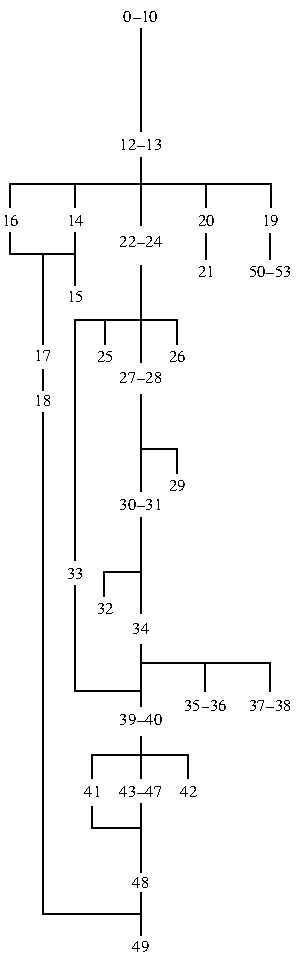
\includegraphics[width=0.409\linewidth,height=.8\textheight,keepaspectratio]{assets/front_dependence_chart.pdf}\end{center}
\begin{center}\textbf{Dependence Chart}\end{center}
\end{BookFloat}

\noindent with the basic material, I give approximately ten pop quizzes per semester that typically involve stating a definition, giving an example, or stating a major theorem.

At the University of North Texas, abstract algebra is a two-semester sequence. The first semester is required of all math majors and the second semester is optional. Because most students opt not to continue with the second semester, it is not offered every year. When I teach either class, I give three 50-minute in-class exams. With exam reviews and going over completed exams, this leaves approximately 36 class periods for new material.

In the first-semester class, the base material I always cover includes Sections 0-6, 8, 9, 12, 13, and 22-25. I average approximately two class periods per section, so I can usually cover a few more sections. Options I have used for the remaining time include

\end{BookBody}

% Source PDF page 15; original printed page xiv
\BookSource{15}{xiv}
\BookNarrativetrue

\begin{BookBody}

\noindent Sections 14 and 15, Sections 26-28, Section 17, or Sections 30 and 31. One semester I attempted to cover enough field extension material in order to cover Section 41. This required me to carefully select material in Sections 27, 28, 39, and 40 in order to prepare the students for Section 41.

For the second semester, I usually have as goals proving the impossibility of bisecting an angle using compass and straightedge and the insolvability of quintic polynomials. Assuming that students have seen the basic material in the first semester as described above, these goals require covering material from Sections 16, 18, 27, 28, 30, 31, 33, 34, and 39-49. This turns out to be an ambitious undertaking, but the purpose of rewriting Part IX was to make the material more accessible to students, and therefore make the goal of covering Galois Theory in a second-semester class more feasible.

\BookTextHeading{\textbf{Acknowledgments}}

\noindent I am very grateful to those who have reviewed the text or who have sent suggestions and corrections. Below is a list of faculty who contributed their thoughts on improving the text.

\BookBullet{Deb Bergstrand, Swarthmore College}

\BookBullet{Anthony E. Clement, Brooklyn College}

\BookBullet{Richard M. Green, University of Colorado}

\BookBullet{Cheryl Grood, Swarthmore College}

\BookBullet{Gary Gordon, Lafayette College}

\BookBullet{John Harding, New Mexico State University}

\BookBullet{Timothy Kohl, Boston University}

\BookBullet{Cristian Lenart, University at Albany, SUNY}

\BookBullet{Mariana Montiel, Georgia Southern University}

\BookBullet{Anne Shiu, Texas A\&M University}

\BookBullet{Mark Stankus, California Polytechnic State University}

\BookBullet{Janet Vassilev, University of New Mexico}

\BookBullet{Cassie L. Williams, James Madison University}

\BookBullet{T. E. Williamson, Montclair State University}

\BookBullet{Michael Zuker, Massachusetts Institute of Technology}

I also wish to express appreciation to Jeff Weidenaar, Tara Corpuz, and Jon Krebs at Pearson for their help with this project.

\noindent Neal Brand

\noindent University of North Texas

\end{BookBody}

% Source PDF page 16; original printed page 
\BookSource{16}{}
\BookNarrativetrue

\begin{BookBody}

\BookTextHeading{\textbf{Student’s Preface}  }

\noindent This course may well require a different approach than those you used in previous mathematics courses. You may have become accustomed to working a homework problem by turning back in the text to find a similar problem, and then just changing some numbers. That may work with a few problems in this text, but it will not work for most of them. This is a subject in which understanding is all-important, and where problems should not be tackled without first studying the text.

Let us make some suggestions on studying the text. Notice that the text bristles with definitions, theorems, corollaries, and examples. The definitions are crucial. We must agree on terminology to make any progress. Sometimes a definition is followed by an example that illustrates the concept. Examples are probably the most important aids in studying the text.\textit{ Pay attention to the examples.}

Before reading a section, it may be helpful to watch the video associated with the section. I have two general pieces of advice for watching a video or reading the text. First, minimize your distractions. It takes a good deal of concentration for most of us to learn new technical information. Second, have paper and pen (or the electronic equivalent) at hand to take notes and to occasionally work out computations on your own.

I suggest you skip the proofs of the theorems on your first reading of a section, unless you are really “gung-ho” on proofs. You should read the statement of the theorem and try to understand just what it means. Often, a theorem is followed or preceded by an example that illustrates it, which is a great aid in really understanding what the theorem says. Pay particular attention to the summary at the end of each video to get an overview of the topics covered.

In summary, on your first viewing and reading of a section, I suggest you concentrate on what information the section gives and on gaining a real understanding of it. If you do not understand what the statement of a theorem means, it will probably be meaningless for you to read the proof.

Proofs are basic to mathematics. After you feel you understand the information given in a section, you should read and try to understand at least some of the proofs. In the videos you will find a few proofs. Watching the videos a second time after you have a better understanding of the definitions and the statements of the theorems will help to clarify these proofs. Proofs of corollaries are usually the easiest ones, for they often follow directly from the theorem. Many of the exercises under the ”Theory” heading 
% Source PDF page 17; original printed page xvi
\BookSource{17}{xvi}
ask for a proof. Try not to be discouraged at the outset. It takes a bit of practice and experience. Proofs in algebra can be more difficult than proofs in geometry and calculus, for there are usually no suggestive pictures that you can draw. Often, a proof falls out easily if you happen to look at just the right expression. Of course, it is hopeless to devise a proof if you do not really understand what it is that you are trying to prove. For example, if an exercise asks you to show that a given thing is a member of a certain set, you must\textit{ know} the defining criterion for a thing to be a member of that set, and then show that your given thing satisfies that criterion.

\end{BookBody}

\BookNarrativetrue

\begin{BookBody}

There are several aids for your study at the back of the text. Of course, you will discover the answers to odd-numbered problems that do not involve a proof. If you run into a notation such as \BookInline{Z_{n}} that you do not understand, look in the list of notations that appears after the bibliography. If you run into terminology like\textit{ inner automorphism} that you do not understand, look in the index for the first page where the term occurs.

In summary, although an understanding of the subject is important in every mathematics course, it is crucial to your performance in this course. May you find it a rewarding experience.

\end{BookBody}
\ifdefined\BookMaster\let\BookFinish\relax\else\def\BookFinish{\end{document}}\fi\BookFinish
